Investigate the performance of \approachshort{} compared to classical \gls{acr:rl} techniques executed on commodity host machines, we see that \Coopfw{} offers a \qtyrange{15}{21}{\times} speedup in median--\num{99.99}\nthscript{th} state-action latency as well as \qty{9.9}{\times} greater online learning throughput.
Crucially, in-\gls{acr:nic} execution offers tight tail latency bounds compared to host-based approaches.
We report on how \approachshort{} scales as additional device resources are added, noting that both in-\gls{acr:nic} designs outperform commodity hosts using just one core in latency and online throughput.
Furthermore, \Indfw{} provides higher per-core offline throughput than host-based approaches, even though our measured hosts exhibit higher clock speeds.
Finally, we show that \approachshort{} has minimal impact on dataplane cross-traffic carried by its parent device.

\subsection{Raw inference and learning performance}\label{sec:opal-results-inference}
\Cref{tab:lats} shows how \approachshort{} compares in latency with a numpy-based \gls{acr:rl} policy.\sidenote{For brevity, I omit numpy-based integer results---against a floating point implementation, median action latencies are \qty{14.6}{\percent} worse, with \qty{7.9}{\percent} longer update times. ??TODO: adapt the table to include these?}
\Coopfw{} achieves sub-\qty{35}{\micro\second} median latency, with \nth{99} and \num{99.99}\nthscript{th} percentile latencies less than \qty{1}{\micro\second} worse using 4 \glspl{acr:me} of the NFP-6480.
This corresponds to \qtylist{15;21}{\times} speedups over a \emph{Collector} host.
Importantly, \Indfw{} achieves lower median state-action latencies (\qty{2.79}{\times}) \emph{and} update times (\qty{2.63}{\times}) than a dedicated \emph{Collector} host while requiring only a single core or dedicated functional unit.

\newlength{\resultplotwidth}
\setlength{\resultplotwidth}{\linewidth}

\begin{table}
	\caption[Latencies and computation times for \approachshort{} versus commodity hardware hosts.]{Latencies and computation times for \approachshort{} versus commodity hardware hosts. On-device execution is crucial in not only lowering latencies, but in reducing tail latencies. Lower is better, with the best marked \emph{in bold}.\label{tab:lats}}
	\resizebox{\linewidth}{!}{
		\expandableinput tables/opal/latency
	}
\end{table}

\begin{table}
	\caption[Action and update throughputs for \approachshort{} versus commodity hardware hosts.]{Action and update throughputs for \approachshort{} versus commodity hardware hosts. Most designs cannot scale online performance with additional cores. Higher is better, with the best marked \emph{in bold}.\label{tab:tputs}}
	\resizebox{\linewidth}{!}{
		\expandableinput tables/opal/tput
	}
\end{table}

\Cref{tab:tputs} compares \approachshort{}'s throughput against host-based execution.
The worker count was chosen for on host machines such that their throughput was maximised without causing latency degradation.
This equalled the amount of physical cores on each device---moving beyond this (even below the number of hyper-threads) would hamper tail latencies by an order of magnitude.
To make the comparison fair in the context of many-core \gls{acr:cpu} environments, we include per-core throughput.
\Indfw{} achieves \qty{2.82}{\times} higher offline throughput than commodity \emph{Collector} hardware in spite of the NFP-6480 having a considerably slower clock speed (\qty{0.29}{\times}).
When compounded with the abundance of such weaker chips, in-\gls{acr:nic} \gls{acr:rl} is able to deliver much higher throughput.
%As anticipated, the \Coopfw{} strategy is key in achieving serviceable throughput in an online learning agent, \qty{9.9}{\times} that of a dedicated collector machine, due to the locking requirements mandating coordinated division of work.
As anticipated, the \Coopfw{} strategy is key in achieving serviceable throughput in an online learning agent, \qty{9.9}{\times} that of a dedicated collector machine, as the write lock around policy updates creates a bottleneck.

By limiting the available workers in software, I show how \Coopfw{}'s policy update time (thus  online throughput---\cref{fig:vary-core}) and state-action latency (\cref{fig:vary-core-latency}) scale with available cores.
While \Coopfw{} always outperforms the host-based floating point implementations, we observe that there are two distinct crossover points which must be met to overcome our own \Indfw{}; \num{8} workers for online throughput, and \num{3} workers for state-action latency.
Some artefacts of the hardware environment and design choices are visible, such as the addition of new physical cores being more significant than contexts, and the presence of some schedule bottlenecks.
Most importantly however, \Coopfw{}'s resource demand is tunable at compile time to meet the online training rate and/or action latency required by a task/environment.

\begin{figure}
	\resizebox{\resultplotwidth}{!}{
		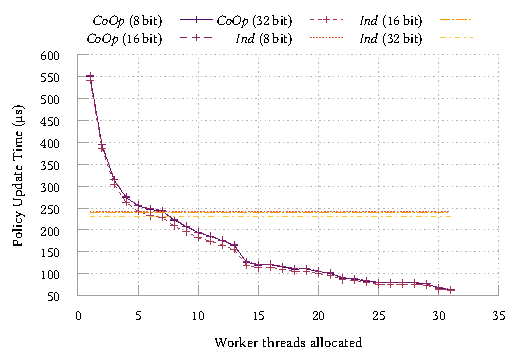
\includegraphics{plots/opal/rl-perf-tester/vary-core}
	}
	\caption[\approachshort{}'s combined update and inference time as the degree of parallelism is varied.]{
		\approachshort{}'s combined update and inference time as the degree of parallelism is varied. \Coopfw{}'s online learning performance improves with additional cores, on max size tasks (\num{129} work items). This requires \num{8} workers to offer greater online throughput than single-threaded in-\gls{acr:nic} \gls{acr:rl}. Sharper performance increases occur when a new physical core is added (\numrange{7}{8}) or the scheduler works around a bottleneck (\numrange{13}{14}).\label{fig:vary-core}}
\end{figure}

\begin{figure}
	\resizebox{\resultplotwidth}{!}{
		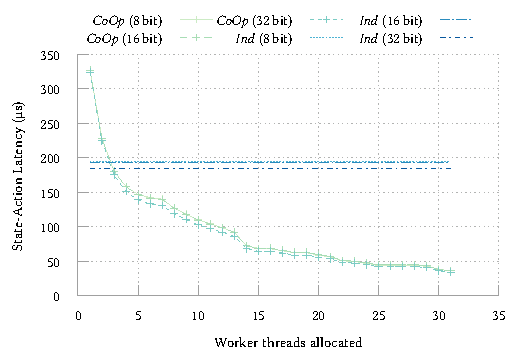
\includegraphics{plots/opal/rl-perf-tester/vary-core-latency}
	}
	\caption[\approachshort{}'s state-action latency as the degree of parallelism is varied.]{\approachshort{}'s state-action latency as the degree of parallelism is varied. \Coopfw{}'s action latencies similarly improve with more cores. This requires \num{3} workers (4 total contexts) to improve upon the state-action latency of single-threaded in-\gls{acr:nic} \gls{acr:rl}.\label{fig:vary-core-latency}}
\end{figure}

\Cref{fig:vary-work,fig:vary-work-latency} show how policy complexity affects update cost and state-action latency respectively, scaling from a bias tile up to the full \gls{acr:ddos} policy size.\sidenote{Input vectors here all have 20 elements regardless of the policy design.}
\Coopfw{} always produces an action in less time than \Indfw{}, but requires at least one state-based tile to excel in online learning.
%We note that this is a trivial case, in that the use of \emph{only} a bias tile negates the need for any input state (similar to a multi-arm bandit problem).
We note that this is a trivial case, as using \emph{only} a bias tile returns a single preference list regardless of input state.

A key aspect of in-\gls{acr:nic} execution is that it allows far tighter bounds on tail latency compared to host inference.
Examining the state-action latencies in \cref{tab:lats}, we see that \num{99.99}\nthscript{th} percentile latencies exceed the median by \qtylist{0.58;0.66}{\percent} for \Indfw{} and \Coopfw{}, respectively.
Similar results were observed for other bit depths.
By contrast, host-based tail latencies are at least \qty{40.53}{\percent} greater even when the parallel worker count is at or below the physical core count.
We show the cumulative distributions of these in detail (\cref{fig:lat-cumul}), noting how just one additional \gls{acr:cpu}-intensive task---potentially automated system updates, scans, or another \gls{acr:vnf}/traffic processing task---impacts tail latencies further (\emph{Float(Over)}).

\begin{figure}
	\resizebox{\resultplotwidth}{!}{
		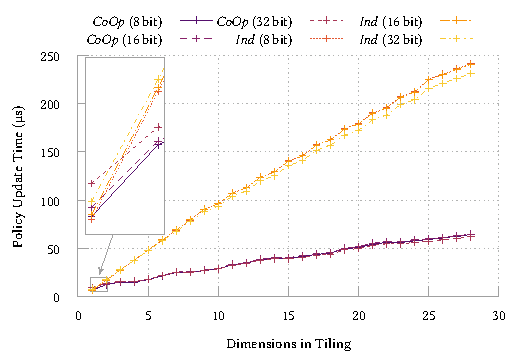
\includegraphics{plots/opal/rl-perf-tester/vary-work}
	}
	\caption[\approachshort{}'s combined update and inference time as the number of tiling dimensions is varied.]{\approachshort{}'s combined update and inference time as the number of tiling dimensions is varied. \Coopfw{} fully processes updates faster than \Indfw{}---thus has higher online performance---on almost all policy sizes. Lower bit depths are more effective on simpler policies.\label{fig:vary-work}}
\end{figure}

\begin{figure}
	\resizebox{\resultplotwidth}{!}{
		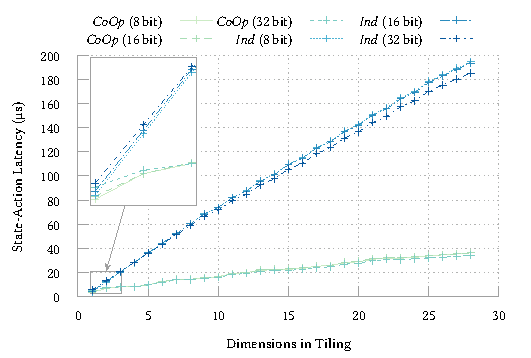
\includegraphics{plots/opal/rl-perf-tester/vary-work-latency}
	}
	\caption[\approachshort{}'s state-action latency as the number of tiling dimensions is varied.]{\approachshort{}'s state-action latency as the number of tiling dimensions is varied. State-action latency scales with additional work in a similar manner to overall processing time; though \qty{32}{\bit} firmwares become more effective sooner (at \num{3} input dimensions, or \num{17} tasks).\label{fig:vary-work-latency}}
\end{figure}

\begin{figure}
	\centering
	\begin{subfigure}{\linewidth}
		\resizebox{1.0\linewidth}{!}{
			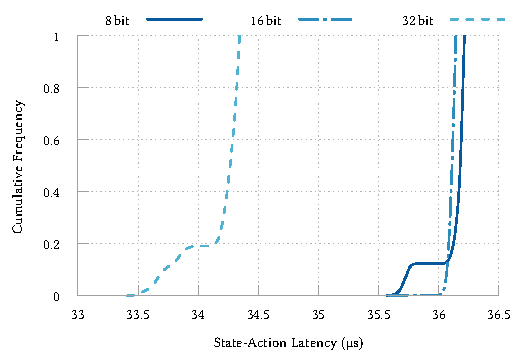
\includegraphics{plots/opal/rl-perf-tester/latency-cumul-thesis}
		}
		\caption{\approachshort's \Coopfw{} design achieves consistent, tight latency bounds, with less than \qty{1}{\micro\second} between minima and maxima for all choices of bit depth. In most cases, latencies follow 32$<$16$<$\qty{8}{bit}.}
	\end{subfigure}

	\begin{subfigure}{\linewidth}
		\resizebox{1.0\linewidth}{!}{
			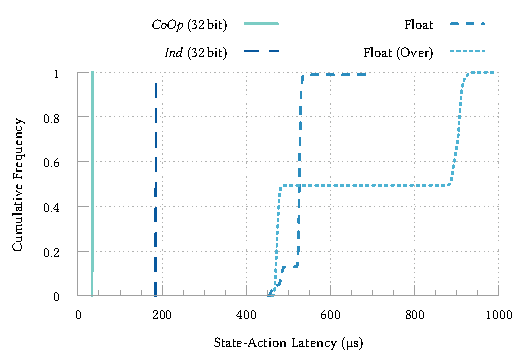
\includegraphics{plots/opal/rl-perf-tester/latency-cumul-broad-thesis}
		}
		\caption{\indfw{} observes higher---though similarly tightly bounded---latencies than \coopfw. In hosts tail latencies suffer, particularly when oversubscribed.}
	\end{subfigure}
	\caption[Cumulative state-action latency plots for \approachshort{} and host-based execution.]{Cumulative state-action latency plots for \approachshort{} and host-based execution. In-\gls{acr:nic} execution offers lower latencies and more consistent latencies than execution on a numpy-based host. \qty{32}{\bit} inference is the lowest-latency strategy in \approachshort{}.\label{fig:lat-cumul}}
\end{figure}

A noteworthy trend is that \qtylist{8;16}{\bit} versions of \approachshort{} consistently underperform compared to \qty{32}{\bit}, except for smaller workloads (seen in the zoomed portions of \cref{fig:vary-work,fig:vary-work-latency}).
This occurs even though our implementation is optimised to read and write policy data in batches (achieving fewer I/O operations).
We see this because the native register width on the \gls{acr:nfp} is \qty{32}{\bit}, and so the compiler must emit extra instructions around arithmetic operations to correctly load and update values.
This matches \qty{32}{\bit} becoming dominant in complex workloads: higher dimension tilings require more arithmetic operations.
Most of the I/O comes \emph{after} this step, causing \gls{acr:alu} use to dominate.
This also explains why \qty{32}{\bit} becomes the best choice at different policy complexities for online (\cref{fig:vary-work}, 10 dims) and offline (\cref{fig:vary-work-latency}, 3 dims) agents, where hashtable accesses and a \texttt{memcpy} of the state vector fall into the serial portion of the online algorithm.
Smaller bit depths still give a \qtyrange{2}{4}{\times} saving in memory for policy storage (enabling more fine-grained or complex policies), in exchange for slightly worse latency and throughput.
To overcome this, we investigated \gls{acr:simd}-like bit-stuffing of values into a single word during atomic writeback (as the platform offers both \qtylist{32;64
}{\bit} atomic addition) as presented in \cref{sec:intra-agent-communication}.
Unfortunately, manipulating tiles into the correct format added \qty{10}{\percent} extra overhead.

\subsection{Work allocation}\label{sec:opal-results-work-alloc}
\Cref{fig:work-alloc-32} shows that our heuristic allocator (\emph{Balanced}) is key in achieving consistent sub-\qtylist{35;65}{\micro\second} latencies and update times, respectively.
The trend is repeated for all bit depths.
The constant difference between \emph{Action} and \emph{Update Prep} scales with bit depth, matching storage and lookup work in the serial portion of \emph{ParSa} (\cref{fig:work-alloc-allbit}).
The severe underperformance of the \emph{Na\"{i}ve} allocator confirms that work item complexity is correlated with its index, as batching work in contiguous chunks gives some workers only high-dimensionality tilings.
The minor gap in lower bound performance between the \emph{Random} and \emph{Balanced} allocators suggests that further optimisations can be made.
We expect that closing or exceeding this gap may require more complex modelling of hardware thread interactions, which lies far beyond the scope of in-NIC scheduling.
Some additional complexity may be tolerated, subject to code store limits---scheduling runs exactly once per configuration change, so does not impact per-action code.

\begin{figure}
	\resizebox{\resultplotwidth}{!}{
		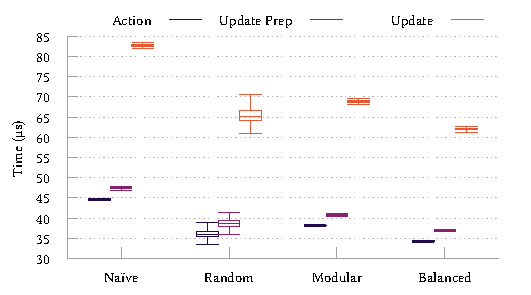
\includegraphics{plots/opal/rl-perf-tester/work-strat-32bit}
	}
	\caption[Action and update compute times in a \qty{32}{\bit} \Coopfw{} agent under different work schedulers.]{Action and update compute times in a \qty{32}{\bit} \Coopfw{} agent under different work schedulers. The \emph{Na\"{i}ve} and \emph{Modular} schedulers achieve worse performance than \emph{Random}'s median value. The \emph{Balanced} scheduler introduced in \cref{alg:parsa-schedule} outperforms these and achieves tight latency bounds while outperforming the expected random schedule. However, there is still a slight performance gap between the empirically observed minimum cost and \emph{Balanced}.\label{fig:work-alloc-32}}
\end{figure}

\begin{figure}
	\resizebox{\resultplotwidth}{!}{
		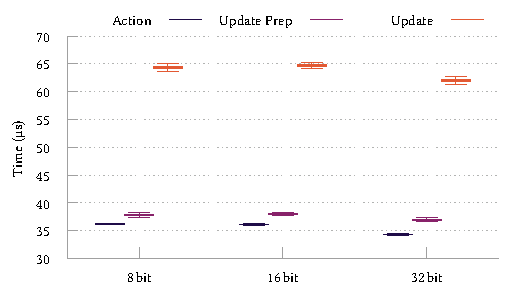
\includegraphics{plots/opal/rl-perf-tester/work-strat-balanced}
	}
	\caption[Stage times of \approachshort's \emph{Balanced} allocator at \qtylist{8;16;32}{\bit} depths.]{Stage times of \approachshort's \emph{Balanced} allocator at \qtylist{8;16;32}{\bit} depths. While the core inference and update logic becomes more efficient at higher bit depths, the logic in the post-inference serial portion (i.e., \emph{Action}$\rightarrow$\emph{Update Prep}) becomes marginally less taxing at smaller bit depths. These serial portions consume \qtylist{1.653;1.907;2.653}{\micro\second} for \qtylist{8;16;32}{\bit} respectively.\label{fig:work-alloc-allbit}}
\end{figure}

\begin{figure}
	\resizebox{\resultplotwidth}{!}{
		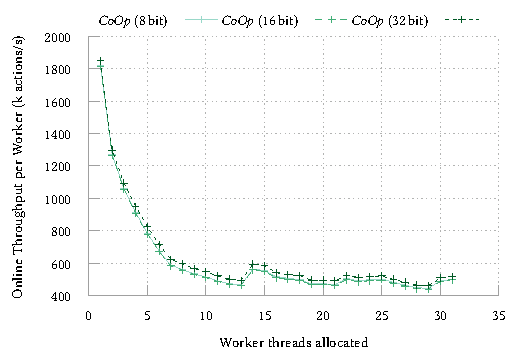
\includegraphics{plots/opal/rl-perf-tester/vary-core-tput-on-per}
	}
	\caption[\approachshort{}-\coopfw{}'s online throughput per core as the number of worker threads is varied.]{\approachshort{}-\coopfw{} online throughput per core as the number of worker threads is varied. Additional threads exhibit diminishing return on overall throughput for a given policy size. Note that the spikes of increasing per-core value correspond to the scheduler bottlenecks observed in \cref{fig:vary-core}.\label{fig:tput-per-core}}
\end{figure}

An interesting aspect of \Coopfw{} and \emph{ParSa} is that adding cores has both diminishing returns and key thresholds to pass.
Consider \cref{fig:tput-per-core}, where the throughput per worker decreases with cores but occasionally increases sharply.
Later downward ticks (\numrange{25}{29} workers) correspond to plateaus in throughput.
This is a problem stemming from the granularity of work items (i.e., tilings in \emph{ParSa}), where our scheduler cannot find a better solution to a bottleneck until extra cores are allocated.
We measured individual work items in state-action computation to take a mean \qtylist{5.2; 6.2; 9.7; 11.0}{\micro\second} for bias, CLS, CTM and IMEM tilings respectively.
Though we have a \qty{4.2}{\times} factor of task oversubscription, it is clear that latencies are eventually bound below by the length of the longest task.

\subsection{End-to-end RL latency}
%?? PCIe RTT is 10us (neugebauer, BNN NFP paper), NFP RTT is 18us (own measurements). EMEM Ring one-way is 120ns.
%?? Cziva~\parencite[pp.113]{DBLP:phd/ethos/Cziva18} discusses vNF times.
%?? reference the inference times brought up in Taurus?
Referring to \cref{fig:state-slip}, we take $t_2$ from \cref{tab:lats} for host and in-\gls{acr:nic} processing times, and substitute $t_1+t_3$ for the state packet round-trip time to the decision site:
\begin{description}
	\item[In-\gls{acr:nic}.] As described in \cref{sec:agent-environment-communication}, EMEM rings have a median one way delay cross-island of \qty{140}{\nano\second}, giving a \emph{median \qty{34.63}{\micro\second} end-to-end inference latency}.
	\item[Dedicated Collector.] Offloads hosted in this manner will employ DPDK to maximise performance, giving one-way \gls{acr:pcie} delays of \qtyrange{0.9}{2.3}{\micro\second} for network packets~\parencite{DBLP:conf/sigcomm/NeugebauerAZAL018}.
	A \gls{acr:udp} packet carrying \num{20} elements of state in \approachshort{} is \qty{128}{\byte}, so costs \qty{1}{\micro\second} to forward, and the reply state-action pair is slightly larger.
	\emph{This gives an end-to-end inference latency of \qty{517.9}{\micro\second}}.
	\item[\gls{acr:vnf} Offload.] \Textcite{DBLP:journals/cm/CzivaP17} show that more lightweight \gls{acr:vnf} frameworks like GNF~\parencite{DBLP:journals/cm/CzivaP17} and ClickOS~\parencite{DBLP:conf/nsdi/MartinsAROHBH14} add \qtyrange{45}{55}{\micro\second} \emph{additional} \gls{acr:rtt} latency above \gls{acr:pcie} costs.
	\emph{This gives an end-to-end inference latency of \qty{572.9}{\micro\second}}.
\end{description}
Using these estimates, in-\gls{acr:nic} classical \gls{acr:rl} inference offers \qtylist{14.96;16.54}{\times} speedups in latency over collector and \gls{acr:vnf} deployments respectively (assuming no steering cost in either case).
We also contrast these against deep RL policies on network tasks, which can take \qty{3}{\milli\second} to compute~\parencite{DBLP:journals/corr/abs-1910-04054}---2 orders of magnitude above \approachshort{} with identically sized (20-dim) input vectors.
%In the name of fairness, we assume that rule installation uses same mechanism we recommend, but show how bad it can get? I.e. with rule installation costs etc.

\subsection{Co-existence with the dataplane}
Our setup met \qty{40}{\giga\bit\per\second} for packet sizes $\ge$\qty{256}{\byte}.
%For frame sizes of \qtylist{64;128;256}{\byte} input traffic rates were \qtylist{17.4;32.9;37.0}{\giga\bit\per\second} respectively (\qtylist[per-symbol=p,sticky-per=true]{33.9;32.2;18.1}{\mega\packet\per\second}).
For frame sizes of \qtylist{64;128}{\byte}, input traffic rates were \qtylist{17.4;32.9}{\giga\bit\per\second} respectively (\qtylist[per-symbol=p,sticky-per=true]{33.9;32.2}{\mega\packet\per\second}).
Passing this traffic over the \gls{acr:nfp} device running \approachshort, no packet losses were incurred at any rate of \gls{acr:rl} actions.

We show the effect of \gls{acr:rl} workloads on the round-trip latencies of cross traffic through \cref{fig:dataplane-heat}.
As observed latencies do not obey a normal distribution (particularly \qtylist{256;1518}{\byte}, which are bimodal), we employ a one-tailed \emph{Mann-Whitney U test} to mark statistically significant population increases in latency ($p < 0.05$) with a ``+''.
In general, statistically significant latency increases concentrate around smaller packet sizes.
All (bar one) of these affected \nth{99} percentile latencies by under \qty{0.38}{\percent} (at most \qty{78}{\nano\second}).
This slight degradation can be explained by increased pressure on the \gls{acr:nfp}'s \gls{acr:cpp} bus, which is responsible for handling cross-island accesses to memory (particularly IMEM/EMEM) and other resources.
\approachshort{} places load on the \gls{acr:cpp} bus through its \inring{}/\outring{} EMEM rings and last-tier policy accesses.
This also explains the sensitivity of \qty{256}{\byte} packets to \approachshort{}---the \gls{acr:nfp} P4 toolchain segments packets, storing metadata (e.g., MAC prepend) and the first bytes of a packet in a \qty{256}{\byte} CTM block and parking their payloads in EMEM.
\qty{256}{\byte} packets overshoot this due to metadata, causing small I/O accesses at a high rate for packets sized around this cutoff.
%Regardless, this effect is small when observed.

The anomalous result is \qty{128}{\byte} packets at \num{3000} \gls{acr:rl} action/update computations per second, causing a \qty{222}{\nano\second} (\qty{1.18}{\percent}) increase, shown in \cref{fig:dataplane-example}.
This is observed through a shift of some packet latencies from the mode towards the tail, but no other changes in the distribution.
In the above context, we believe that the inbound request rate is weakly synchronised with inbound packets, causing a higher level of burstiness around accesses to the \gls{acr:cpp} bus.
We expect that dedicated hardware or \gls{acr:fpga} designs can avoid this problem by having dedicated \inring{}/\outring{} access mechanisms for an \approachshort{} agent.

\begin{figure}
	\centering
		\resizebox{1.0\linewidth}{!}{
%			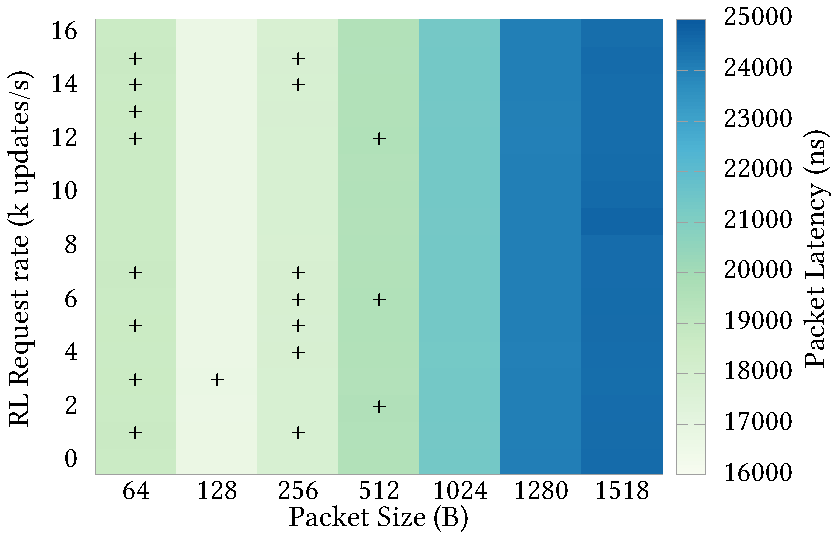
\includegraphics{../plots/build/stress/heat-latency-median}
			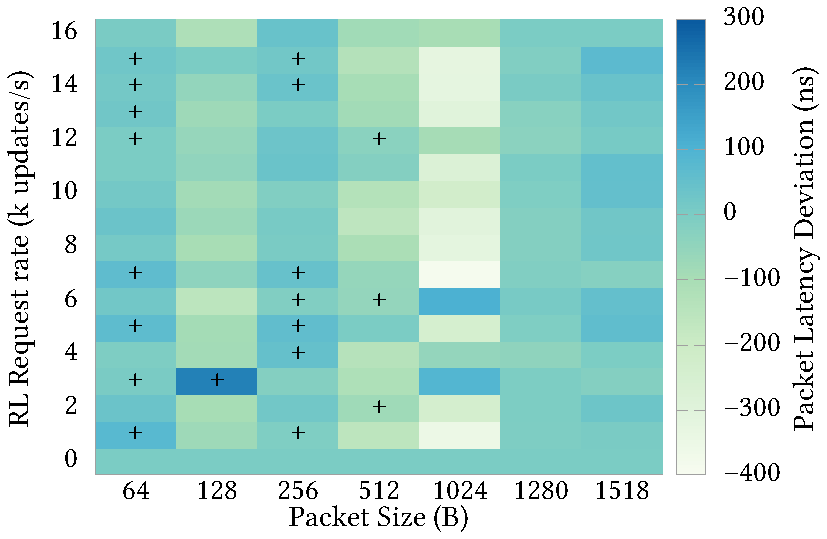
\includegraphics{plots/opal/stress/heat-latency-two-9-rel}
%			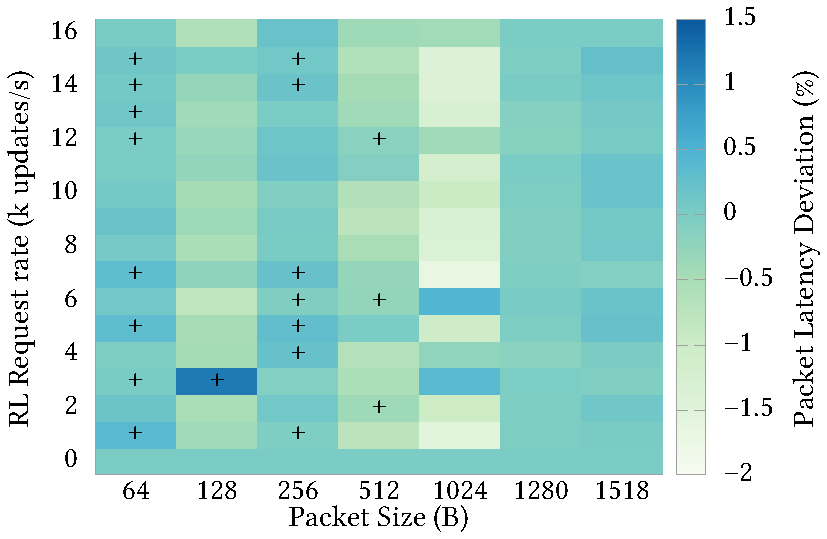
\includegraphics{../plots/build/stress/heat-latency-two-9-perc}
		}
		\caption[Deviations in \nth{99} percentile cross-traffic RTTs for an \approachshort{} agent processing \numrange{0}{16}k updates/s.]{Deviations in \nth{99} percentile cross-traffic \glspl{acr:rtt} for an \approachshort{} agent processing \numrange{0}{16}k updates/s. Statistically significant increases in population latency are marked with a ``+''. These concentrate on smaller packet sizes, and are typically sub-\qty{78}{\nano\second}.\label{fig:dataplane-heat}}
\end{figure}

\begin{figure}
	\centering
		\resizebox{1.0\linewidth}{!}{
			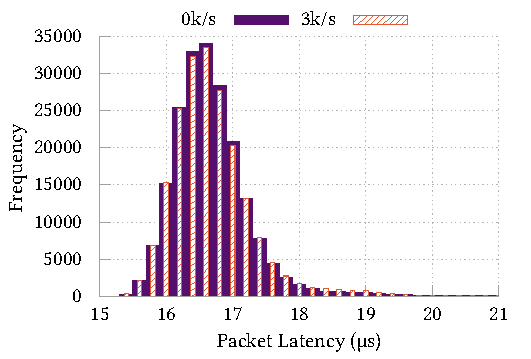
\includegraphics{plots/opal/stress/histo-128B-0-3-up-trim}
		}
		\caption[Distribution of RTTs for \qty{128}{\byte} packets for \numlist{0;3000} full RL updates/s.]{Distribution of \glspl{acr:rtt} for \qty{128}{\byte} packets for \numlist{0;3000} full \gls{acr:rl} updates/s. This is an anomalously high deviation present in \cref{fig:dataplane-heat}---the median value has not altered, but the peak has dampened somewhat, increasing tail latencies.\label{fig:dataplane-example}}
	
%	\caption{Effects on tail latency of cross-traffic caused by different loads of off-path \gls{acr:rl} compute. Statistically significant increases in population latency are concentrated on smaller packet sizes, and are typically sub-\qty{78}{\nano\second}.\label{fig:dataplane-coop}}
\end{figure}

\subsection{Resource requirements}
\Cref{tab:resources} shows how \approachshort{} consumes shared memory as it scales to fit a device's compute resources, compared with a simple P4 forwarding application.
As one program is installed per \gls{acr:me}, these results represent the minimum and maximum resource use on a single island (i.e., without replacing P4 workers).
We observe negligible costs on shared EMEM ($\sim$\qty{4}{\mebi\byte}), incurred due to hashtables for past state and rewards.
The most significant costs arise due to policy data (\qty{405}{\kibi\byte} shared IMEM, \qty{90}{\kibi\byte} local CTM, \qty{15}{\kibi\byte} local CLS), which can be halved or quartered using \qtylist{16;8}{\bit} quantisation and remain constant regardless of compute unit usage.
This is a high upfront cost on per-island resources (CLS/CTM)---\approachshort{} leaves resources for other off-path dataplane applications, but is fairest from 3 cores onwards.

%Thread local storage in CLS for compute/register spilling scales with the number of MEs required (requiring \qtylist{13.77;15.49}{\percent} per-ME for \Indfw{}/\Coopfw) due to precaching and the space needed to hold tile lists.
%Due to the initial policy cost this falls below the fair share at 3 MEs, but always allows for co-existence with other asynchronous dataplane programs.

\begin{table}
\caption[NFP memory incurred by \approachshort{} when built to use \numlist{1;4} MEs (\qty{32}{\bit}).]{\gls{acr:nfp} memory incurred by \approachshort{} when built to use \numlist{1;4} \glspl{acr:me} (\qty{32}{\bit}). CLS and CTM are shared between all programs on the same island (placing our \gls{acr:rl} agent on i5), while EMEM and IMEM are shared between all \gls{acr:nfp} programs on a \gls{acr:nic}.\label{tab:resources}}
\resizebox{\linewidth}{!}{
\begin{tabular}{
		@{}c
		S[table-format=4.2] S[table-format=2.2]
		S[table-format=4.2] S[table-format=2.2]
		S[table-format=4.2] S[table-format=2.2]
		S[table-format=2.2] S[table-format=2.2]
		S[table-format=3.2] S[table-format=2.2]
		@{}
	}
	\toprule Firmware & \multicolumn{2}{c}{EMEM} & \multicolumn{2}{c}{EMEM Cache} & \multicolumn{2}{c}{IMEM} & \multicolumn{2}{c}{i5.CLS} & \multicolumn{2}{c}{i5.CTM}\\
	& \multicolumn{1}{c}{\si{\mebi\byte}} & \multicolumn{1}{c}{\si{\percent}} & \multicolumn{1}{c}{\si{\kibi\byte}} & \multicolumn{1}{c}{\si{\percent}} & \multicolumn{1}{c}{\si{\kibi\byte}} & \multicolumn{1}{c}{\si{\percent}} & \multicolumn{1}{c}{\si{\kibi\byte}} & \multicolumn{1}{c}{\si{\percent}} & \multicolumn{1}{c}{\si{\kibi\byte}} & \multicolumn{1}{c}{\si{\percent}} \\
	\midrule Base P4 & 6776.67 & 88.24 & 268.52 & 2.91 & 858.28 & 10.48 & 0.00 & 0.00 & 0.00 & 0.00 \\
	\Indfw(1) & 6780.21 & 88.28 & 2541.08 & 27.57 & 1263.28 & 15.42 & 24.75 & 38.67 & 94.25 & 36.82 \\
	\Indfw(4) & 6780.22 & 88.28 & 2545.33 & 27.62 & 1263.28 & 15.42 & 51.18 & 79.97 & 107.00 & 41.80 \\
	\Coopfw(1) & 6779.12 & 88.27 & 1773.59 & 19.24 & 1263.28 & 15.42 & 22.41 & 35.01 & 90.00 & 35.16 \\
	\Coopfw(4) & 6779.12 & 88.27 & 1769.84 & 19.20 & 1263.28 & 15.42 & 52.16 & 81.49 & 90.00 & 35.16 \\
	\bottomrule
\end{tabular}
}
\end{table}

%\paragraph{The impact of bit depth}
%?? \Cref{fig:quant-acc}
%?? \qty{5}{\bit} mantissa suffices for $\ge$ \qty{90}{\percent} relative accuracy, so \qty{8}{\bit} is fine (1S + 2E + 5M), \qty{16}{\bit} is better.
%
%\begin{figure}
%	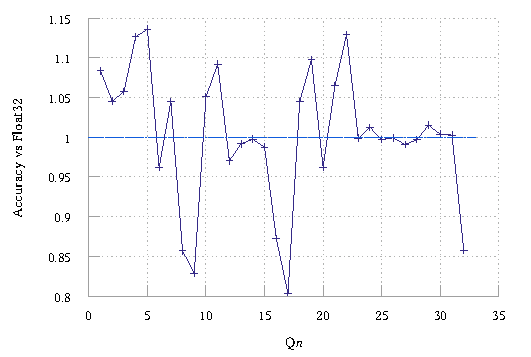
\includegraphics{../plots/build/marl-quant/accuracy-binary}
%	\caption{Normalised accuracy of a converted, pre-trained floating-point tile-coded policy after conversion to $32Qn$ fixed-point.}\label{fig:quant-acc}
%\end{figure}

\subsection{Deployability}
Setup of \approachshort{} uses two packet types: \emph{setup}, which contains learning parameters, hyperparameters, and most aspects of a policy, and \emph{tiling}, which provides a list of state indices for tiling sets.
Instrumentation in \approachshort{} found that setup and tiling packets take a mean \qtylist{27.03;16.69}{\micro\second} to be processed on \Indfw{}, allowing an agent to be swapped between online and offline operation (or repurposed for another task) painlessly.
Online/offline swaps are useful when an agent should cease learning (i.e., when performance has converged), or if a change in the environment suggests that more training is needed.
Tiling packet processing scales linearly with the number of \emph{tiling sets}, due to the needed precaching of tile set boundaries.
Online-offline swaps for \Coopfw{} exhibit similar cost, however the need for explicit scheduling means that policy/tiling \emph{structure} changes (including the first complete setup) take \qty{422.63}{\micro\second} for the full-size policy described above.
The time taken for \Coopfw{} to schedule its tasks was found to scale with the number of workers ($m$) and work items ($n$) as described earlier (\cref{sec:work-allocation}, $\mathcal{O}{\left(n\log{m}\right)}$).
Ignoring the trivial solutions, reducing the worker count to \num{1} costs a mean \qty{238.22}{\micro\second}, while placing a single task incurs \qty{53.79}{\micro\second}.
Policy \emph{data} changes require no additional work in any case, resolving purely to \texttt{memcpy}s.

Firmware (re-)installation (i.e., changing from \Indfw{} to \Coopfw{}, bit depth, or increasing maximum policy sizes) took a mean time of \qty{38.83}{\second}.
In the event that appropriate firmwares are not pre-compiled, we found that compiling and linking both \approachshort{} and the P4 toolchain took around \qty{35}{\second}, while changing only \approachshort{} parameters required around \qty{25}{\second}.
These results show that \approachshort{} can be easily adapted and altered by network administrators once in place, and illustrates an advantage of \gls{acr:soc}-based SmartNICs.

\subsection{Magnitude comparisons against PDP ML}
Full, in-network packet tagging and classification by pre-trained \glspl{acr:bnn} is shown by \emph{N3IC}~\parencite{DBLP:journals/corr/abs-2009-02353}.
N3IC achieves packet inference in \qty{45}{\micro\second} on the \gls{acr:nfp}, and \qty{0.3}{\micro\second} on NetFPGA for \qty{256}{\bit} inputs.
Comparatively, \approachshort{}-\Coopfw{} can process an identically-sized input (8-dim) in a median \qty{13.83}{\micro\second}.
This work handles larger inputs (\qty{640}{\bit}) at lower latencies (\qty{34}{\micro\second}), and offers online learning.
We expect that a NetFPGA implementation of \approachshort{} would enjoy a similar factor of speedup.
No works investigate the runtime training of \gls{acr:bnn} function approximators in-\gls{acr:nic}.

\textcite{langlet-ml-netronome} has shown the viability of \gls{acr:nn} inference using \qty{64}{\bit} quantisation on the \gls{acr:nfp}, using \emph{in-path} compute rather than our asynchronous model.
Inference latency on small networks (3 layers, \num{30} neurons) can be as high as \qty{500}{\micro\second} on line rate traffic using \qty{2304}{\bit} inputs, emphasising the value of path-adjacent compute.

Taurus~\parencite{DBLP:journals/corr/abs-2002-08987} proposes that efficient line-rate inference can be achieved using a configurable grid of map-reduce units in the packet pipeline (implementing e.g., \glspl{acr:lstm} and \glspl{acr:svm}).
On \gls{acr:cgra} hardware, they achieve sub-\si{\micro\second} extra latency for inputs of an unclear size.
\emph{IIsy}~\parencite{DBLP:conf/hotnets/XiongZ19} shows how \emph{classical \gls{acr:ml} inference} (\glspl{acr:svm}, Na\"{i}ve Bayes, etc.) can be converted into match-action tables compatible with \emph{any} P4 deployment.
They achieve mean \qty{2.62}{\micro\second} extra in-path latency on NetFPGA (at line rate in most cases) on \qty{59}{\bit} inputs when illegal values are excluded.
As these approaches are reliant on specialised hardware-accelerated primitives for inference, an apples-to-apples comparison is difficult.
However by considering the relative performance of N3IC between Netronome and \gls{acr:fpga} implementations it is reasonable to place N3IC (and thus \approachshort{}) in the same performance band.